\documentclass{article}
\usepackage[utf8]{inputenc}
\usepackage{authblk}
\usepackage{color}
\usepackage{graphicx}
\usepackage{todonotes}


%\newcommand{\note}[1]{\textcolor{red}{#1}\xspace}
\newcommand{\note}[1]{\textcolor{red}{#1}}
\author[1, 2]{David Robinson}
\author[1, 2]{Miles Currie}
\author[1, 2]{Bryan Quaife}
\author[1]{Kevin Speer}

\affil[1]{Geophysical Fluid Dynamics Institute}
\affil[2]{FSU Department of Scientific Computing}

\title{CAndbox: Modeling Fire Spread on Real-Time Interactive Terrain}
\date{}

\begin{document}


\maketitle

\begin{abstract}
Modeling the spread of forest fires via cellular automata is an attractive approach for its efficient computational implementation, and the surprising realism of deceptively simple algorithms in simple geometries. However, applying this method to a real wildland fire environment with complex fuel, topography, and wind requires substantial parameterization. An established approach is to use pixel-by-pixel rates of spread derived from the Rothermel model, but these models do not integrate over the contributions of multiple ignited pixels and only allow a discrete number of states. We present a new method which allows for semi-discrete states by summing over the contribution of all ignited pixels on a combustable pixel within a given neighborhood. Folding together the effects of terrain and wind speed, we employ an extended Rothermel model to form an ``effective spread ellipse'' defined by the rate of spread an ignited pixel contributes in any direction. Furthermore, we tune the model to real fire data using Bayesian inference. Because of the computational efficiency of this method, we are able to apply it to a “sandbox", an augmented reality projection system. Initially designed to demonstrate fluid flow on an evolvable surface, this system allows the fire model to facilitate real-time adjustments to topography and burning regions. Additionally, the system handles complex initial fire shapes while remaining intuitive to the user. The outcome is a tool that is ideal for exploring the effect of topography on the spread rates of fire in a real-time environment.

\end{abstract}


\section{Introduction}
This is the introduction

\section{Model}

\subsection{Modification to Previous Model}

\subsubsection{Previous Model}

\subsubsection{Our Model}


\begin{itemize}
\item Based on rothermel model
\item explain classical approach
\item explain fire bucket method and how it differs
\end{itemize}

We use the Rothermel model given by

\begin{equation}
\label{eq:rothermel}
R(\theta) = R_0 \frac{1-\overline{E}}{1 -\overline{E}\cos(\theta) }
\end{equation}
where $\theta$ is the angle measured from the direction of maximum spread, $R_0$ is the rate of spread with no wind or terrain effects, and $\overline{E}$ is the ellipse eccentricity, defined as
\begin{equation}
\label{eq:ebar}
\overline{E} = \sqrt{1 - 1/LW^2}
\end{equation}
where LW is the ellipse length-to-width ratio calculated as 
\begin{equation}
\label{eq:lw}
LW =  0.936 e^{0.2566U_{eq}} + 0.461e^{-0.1548U_{eq}} - 0.397
\end{equation}
where the equivalent wind speed $U_{eq}$ ($\frac{m}{s}$) is the wind speed that alone would produce the combined effect of actual wind and terrain slope. 

Our CA method uses the Rothermel model to draw an ellipse around a single ignited cell, where the cell in question is one of the foci. $R(\theta)$ gives the rate of spread around the cell as an ellipse. 

{\bf Outline of code:}
\begin{itemize}
\item the code is based on a grid system:
\item grid for terrain (elevation), wind direction, wind speed, a state grid, a bucket grid, and a fuel grid
\item explain each of these
\item explain states
\item we have timesteps:
\item for each timestep, we find the cells in the ``I'', or burning state
\item for each of the cells in the ``I'' state, we first check to see if they can be extinguished-- how?
\item then, several steps:
\item for a burning cell, we find the elevations of its eight neighbors and calculate the slope between each neighbor and the cell of interest
\item we then find the rate of spread from the Rothermel model with inputs of fuel, wind magnitude, and wind direction
\item then calculate modifications to the rate of spread given by effects of the terrain and wind (phi values, write equations)
\item treat the ros values as contributions to the neighboring cells (maybe show example in a figure?)
\item add these values to bucket grid
\item check where on the bucket grid the buckets are ``filled up''. ie we have some threshold, in the initial case unity, where we call the buckets full and then change the corresponding cell on the state grid to the ``I'' state.
\item do these steps for each timestep
\end{itemize}


\subsection{Grid System}
Our model is based on the use of a grid system: All information is stored in separate grids that describe the terrain, wind magnitude, wind direction, fuel, the state of each cell, and a means to store the contributions of burning cells on others.

\subsubsection{Terrain Grid\label{sec:terraingrid}}
To describe the terrain, our model requires a grid of elevation values at each cell. The elevation values are used to calculate a slope between a cell of interest and its neighbors. The slope information contributes to the rate of spread. 

\subsubsection{Wind Grids\label{sec:windgrid}}
Although wind can be described by a single grid of vectors, we found it is simpler to describe wind in two separate grids, one for magnitude and the other for direction. This works better with the software we use for projecting this model onto our sand box because each texture requires a single value for each cell, which would not work for a vector. \note{(David, is this right? Please correct me if I got it wrong.)}

\subsubsection{Fuel Grid\label{sec:fuelgrid}}
Each cell is able to carry a different value for the type of fuel present in it. This makes it easy to later add a fuel model in to further compare to other fire models. 

\subsubsection{State Grid}
The state grid stores the present state of each cell. Each cell can only be one of four states:
\begin{itemize}
\item U: the cell is unburnable
\item N: the cell is flammable, but not currently ignited
\item I: the cell is flammable and currently ignited, however the fuel is not yet consumed
\item C: the cell is not currently ignited and all fuel has been consumed
\end{itemize}

Unburnable (U) cells can include objects like rocks or bodies of water and are forbidden to ignite in our simulations. Flammable cells also carry fuel information in the corresponding fuel grid (Section~\ref{sec:fuelgrid}).


\subsubsection{Bucket Grid}
Heavily tied to the state grid, the bucket grid carries the information that tells the state grid when to switch a cell in the ``N'' state to the ``I'' state. For a given cell in the ``I'' state, we determine the ``energy'' contribution of that cell to each of its eight nearest neighbors by employing the Rothermel model (Equation~\ref{eq:rothermel}). This process is further described in Section~\ref{sec:propagation} and Figure~\ref{fig:buckets}.



\subsection{Rate of Spread Calculations}
For each iteration (timestep) of our model, several steps are implemented to propagate the fire wall. We begin by obtaining all cells in the ``I'' state. Cells in any other state are skipped over because the fire is not able to propagate to them. For all cells in the ``I'' state, we first check if they will be extinguished, and if not, we continue with the process of calculating the rate of spread for these cells. 

\subsubsection{Extinguishing Cells}
Following the suggestion of \cite{ghisu15}, a cell is only moved from the ``I'' state to the ``C'' when all eight of its nearest neighbors are in some combination the ``I'', ``C'', and ``U'' states. In other words, if all eight of its neighbors have no potential to light on fire, the cell is moved to the ``C'' state. 

In each timestep, the first action performed after finding all cells in the ``I'' state is determining if any of those cells are switched to the ``C'' state using this algorithm. 

\subsubsection{Fire Propagation\label{sec:propagation}}
For all ``I'' cells which pass the extinguishing algorithm still in the ``I'' state, we begin calculating individual rate of spread ellipses using the Rothermel model. The Rothermel model requires several input parameters, which the are stored in the aforementioned grid system. $R_0$ directly corresponds to the type of fuel present in each cell and is found in the fuel grid (Section~\ref{sec:fuelgrid}). $\overline{E}$ is more complicated, however it can be calculated using Equations~\ref{eq:ebar}~and~\ref{eq:lw}, with $U_{eq}$ coming from the corresponding value in the wind manitude grid. $\theta$ is the angle of a cell's neighbor measured from the direction of maximum spread, or wind direction, which is found in the wind direction grid. 

Because the Rothermel model in Equation~\ref{eq:rothermel} does not include a modification for terrain effects and an arguably weak modification for wind speed \note{(this may not be true)}, we introduce two new parameters that are used in the FARSITE fire model \cite{}, $\Phi_s$ and $\Phi_w$, which describe these effects further:


\begin{equation}
\Phi_s = 5.275\beta^{-0.3}\tan(\phi)^2
\end{equation}
\note{we need to check on the tan value. not sure whether $\phi$ is squared or $\tan(\phi)$ is squared}
\todo[inline]{Where is the squared and why?  What is $\phi$?  Can
$\Phi_s$ ever be negative?  If not, the ROS ellipse will always grow
regardless of the slope which is incorrect.}
\begin{equation}
\Phi_w = C(3.28U)^B\left(\frac{\beta}{\beta_{op}}\right)^{-E}
\end{equation}
\note{$\Phi_w$ is left out of my code at the moment}

where b is the packing ratio of the fuel bed and f is the slope (radians), U is the midflame windspeed ($\frac{m}{s}$), and the C, B, and E coefficients are functions of the fuel particle sizes in the fuel bed \cite{}(Burgan 1987; Rothermel 1972).

Table~\ref{tab:inputsummary} summarizes all input parameters for the Rothermel model and where the algorithm finds them. We input these parameters in the Rothermel model to obtain rate-of-spread valuse for the eight nearest neighbors of a given cell. We treat these values as energy values, filling up the energy buckets in the neighboring cells. Figure~\ref{fig:buckets} shows an example of this with an ellipse of eccentricity $0.5$. The cell in the direction of maximum spread gets the most energy from this ellipse, thus it fills up faster than the rest of its neighbors. The biggest advantage to this method is that neighboring cells also in the ``I'' state can contribute to the ignition of ``N'' cells which share the same neighborhood as other ``I'' cells. 

\begin{figure}
\centering
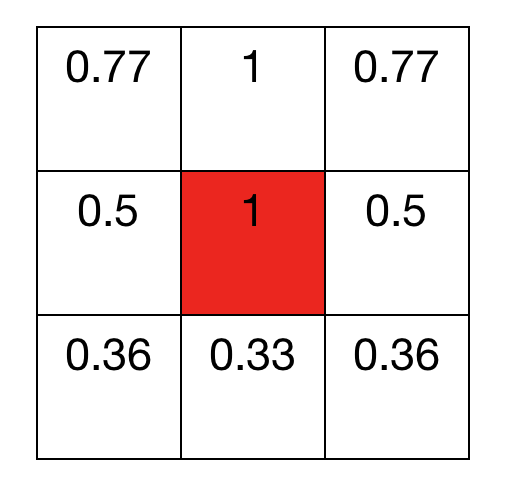
\includegraphics[width=0.6\textwidth]{fire_bucket_ex.png}
\caption{An example of a $0.5$ eccentricity rate-of-spread ellipse's energy contribution on neighboring cells. These values are calculated from Equation~\ref{eq} with $R_0 = 1$ and $\overline{E} = 0.5$ (eccentricity). In this example, and with a combustion threshold of $1$, the cell directly to the north will change states from ``N'' to ``I'' in this timestep. It will be able to make contributions to its respective neighbors in the next timestep. The remaining values are saved and new rate-of-spread values will be added to them in subsequent timesteps until they pass the combustion threshold.\label{fig:buckets}}
\end{figure}

Once cells' energy buckets are filled up to a certain threshold, we change the state of the cell from ``N'' to ``I'' and these cells are able to contribute to their neighbors in subsequent timesteps. After reassigning these states, the process for one timestep is complete and the next timestep begins. 



\begin{table}[h]
\caption{Inputs Summary\label{tab:inputsummary}}
\centering
\begin{tabular}{ |c|c| } 

 \hline
 Model Parameter & Corresponding Grid Parameter \\ 
 \hline
 $R_0$ &  Fuel Grid \\ 
 		         &(\ref{sec:fuelgrid}) \\
 \hline
 $\overline{E}$ &  Wind Magnitude Grid \\ 
 				                     & (\ref{sec:windgrid}) \\
 \hline
 reference angle & Wind Direction Grid \\
 for $\theta$   & (\ref{sec:windgrid}) \\
 \hline
 $\Phi_s$ & Terrain Grid \\
                & (\ref{sec:terraingrid}) \\
  \hline
  $\Phi_w$ & \note{left out at the moment} \\
  \hline
                
  
\end{tabular}


\end{table}

\section{Sandbox}
David
\section{Discussion and Conclusions}

\end{document}
